% To convert to PNG use
% convert -density 300 -transparent white -colorspace RGB output.pdf output.png

\documentclass[border=0.2cm]{standalone}
\usepackage{tikz}

\usetikzlibrary{shapes}
\usetikzlibrary{arrows}
\usetikzlibrary{positioning}
\usetikzlibrary{calc}
\usetikzlibrary{fit}

\tikzset{
	node distance=1.5cm,
	every node/.append style={align=center},
	every path/.append style={->},
	every matrix/.append style={draw, column sep=15, row sep=7},
	var/.style={draw,
		    ellipse,
	    	    minimum height=1.9cm,
	    	    minimum width=3.5cm}
}

\begin{document}

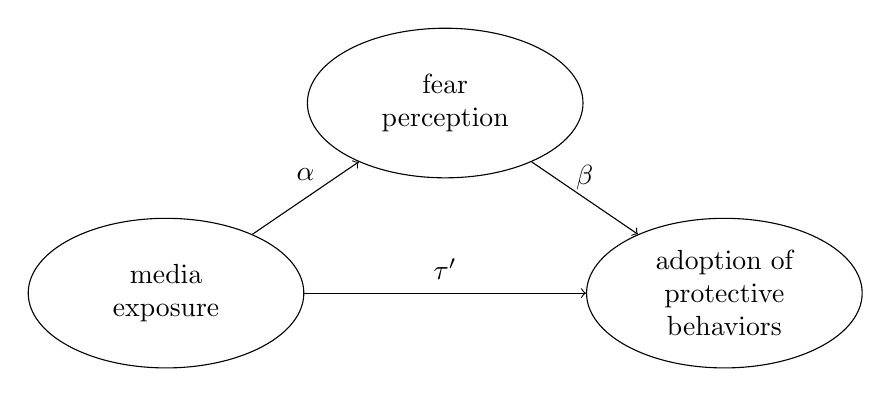
\begin{tikzpicture}
		    
	\node [var] (media) {media\\exposure};
	\node [var, above right=of media] (fear) {fear\\perception};
	\node [var, below right=of fear] (behavior) {adoption of\\protective\\behaviors};

	\path (media) edge node  {$\alpha$ \\[0.5em]} (fear);
	\path (fear) edge node  {$\beta$ \\[0.5em]} (behavior);
	\path (media) edge node  {$\tau'$ \\[0.5em]} (behavior);

\end{tikzpicture}

\end{document}
